\documentclass[a4paper, 10pt, fleqn]{article}
\usepackage{../custom}
\usepackage{../pageformatting}

\usepackage[ngerman]{babel}
%mathe packages
\usepackage{amsmath}
\usepackage{booktabs}
\newcommand{\tabitem}{~~\llap{\textbullet}~~}
\usepackage{tablefootnote}

\graphicspath{{pdf/}{../images/}}

%============PAGE PROPERTIES=============
\newcommand{\revisiondate}{\today}
\newcommand{\documenttitle}{Clock Pendulum Analyzer} % used for title in title and subtitle pages
\newcommand{\authors}{Tobias Kreienbühl \& Daniel Föhn} %used for title page only
\newcommand{\subauthors}{im Auftrag der Hochschule Luzern} %used for title page only
\newcommand{\subtitle}{PMP}%usedfortitleandsubtitlepages
\newcommand{\documentdesc}{Ein Projekt Management Plan für \documenttitle}
\newcommand{\hwb}{Hardware-Board}
\newcommand{\dozent}{Josef Bürgler}
\newcommand{\rpi}{Raspberry Pi 3}
\newcommand{\iic}{$I^2C$}

\begin{document}
	\begin{titlepage}
		\titleGM
		\thispagestyle{empty}
	\end{titlepage}
	
	\tableofcontents
	\listoffigures
	\listoftables
	
	\clearpage
    \section{Einführung}
		\subsection{Zweck des Dokuments}
		\subsection{Zielpublikum}
		\subsection{Versionierung}
			\begin{table}[h]
				\centering
				\begin{tabularx}{\textwidth}{|c|c|X|}
				\hline
				\rowcolor{shadecolor}\textbf{Version} & \textbf{Datum} & \textbf{Kommentar}\\ \hline
				V1.0 & \today & initial file \\ \hline
				\end{tabularx}
			\end{table}
		\subsection{Glossar}
			\begin{description}
				\item[Abkürzung]- Erklärung
			\end{description}

\subtitlepage{Projektmanagement}
	%!TEX root = PMP_ClockPendulumAnalyzer.tex
\section{Projektorganisation}
    Das Projekt besteht aus 2 Entwicklern und einem Product Owner der als Ansprechperson gilt. Dadurch wird die Projektorganisation möglichst klein gehalten. Die Verantwortung wird gleichmässig auf die beiden Entwickler aufgeteilt. Die Abbildung \ref{fig:projektorganisation} gibt einen Überblick.
    \begin{figure}[H]
        \centering
        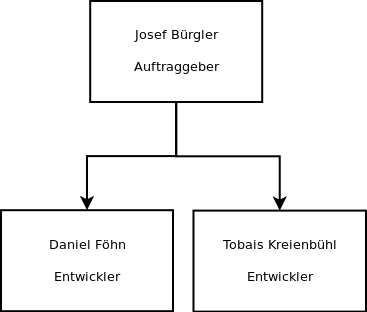
\includegraphics[width=.5\textwidth]{organisation.png}
        \caption{einfache Projektorganisationsstruktur}
        \label{fig:projektorganisation}
    \end{figure}
	\noindent\textbf{Entwickler:} Tobias Kreienbühl
    \begin{itemize}
        \item Projektplanung
        \item Entwicklung der Software C
        \item Entwicklung der Elektronik
        \item Mathematische Umsetzung
    \end{itemize}
    \vspace{.5cm}
    \textbf{Entwickler:} Daniel Föhn
    \begin{itemize}
        \item Projektplanung
        \item Entwicklung der Software C++
        \item Aufbau der System Umgebung
    \end{itemize}
    \vspace{.5cm}
    \textbf{Product Owner / Dozent:} Josef Bürgler
    \begin{itemize}
        \item Anforderungen abnehmen
        \item Entwicklungs-Feedback geben
        \item Projektbetreuung
        \item Coaching
    \end{itemize}
    
    \clearpage
	%!TEX root = PMP_ClockPendulumAnalyzer.tex
\section{Projektrahmenplan}
    In diesem Kapitel werden die Meilensteine und Eckdaten wie Start- und Endzeitpunkt des Projekts festgehalten. In der Abbildung \ref{fig:rahmenplan} ist die Übersicht auf die geplanten Sprints und Meilensteine (MS). Die Meilensteine sowie Abgabetermine sind weiter unten in der Tabelle \ref{tab:meilensteine} ausführlicher beschrieben.
    \begin{figure}[H]
        \centering
        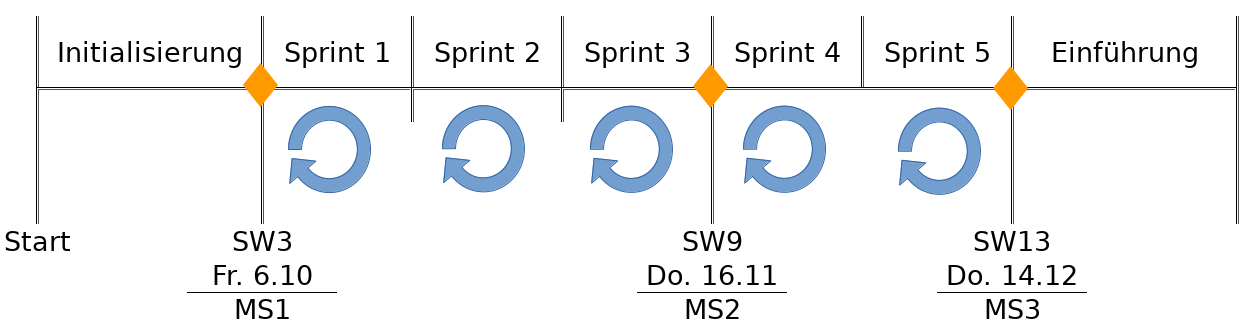
\includegraphics[width=\textwidth]{rahmenplan.png}
        \caption{Rahmenplan mit Phasen, Meilensteine und Sprints}
        \label{fig:rahmenplan}
    \end{figure}
    \begin{table}[h]
        \begin{tabularx}{\textwidth}{lll}
            \textbf{MS1:} & Zeitpunkt: & Freitag 6.10.\\
            & Artefakte: & \tabitem Projekt Management Plan (PMP)\\
            & & \tabitem Entwurf des Grobkonzepts\\
            & Ergebnisse: & \tabitem definierte Vorgehensart\\
            & & \tabitem Rahmenplanung\\
            & & \tabitem Vision (Scope, Ziele etc) im Grobkonzept\\
            \textbf{MS2:} & Zeitpunkt: & Donnerstag 16.11.2017\\
            & Artefakte & \tabitem Prototyp 1\\
            & Ergebnisse: & \tabitem lauffähiger 1. Prototyp\\
            & & \tabitem 80\% der Sys Spec\\
            \textbf{MS3:} & Zeitpunkt: & Donnerstag 14.12.2017\\
            & Artefakte & \tabitem PMP \\
            & & \tabitem SysSpec \\
            & & \tabitem Arbeitsjournal \\
            & & \tabitem Prototyp 2\\
            & Ergebnisse: & \tabitem lauffähiger 2. Prototyp\\
            & & \tabitem fertige System Spezifikation (Projektreport)\\
            & & \tabitem fertiger PMP\\
            \textbf{weitere Termine:} & & \\
            & Abgabe Dokumentation: & 05.01.2018\\
            & Abgabe Projekt: & 12.01.2018\\
            & Präsentation Projekt: & 12.01.2018\\
        \end{tabularx}
        \caption{Meilensteine und Termine}
        \label{tab:meilensteine}
    \end{table}
    
    \clearpage

    \clearpage
    %!TEX root = Projektdokumentation_ClockPendulumAnalyzer.tex
\newcommand*{\risk}[2]{
    \begingroup
    \ifnum #1>#2
    \cellcolor{red}
    \fi
    \endgroup
}

\section{Risikomanagement}
    In diesem Kapitel werden allfällige Risiken identifiziert, bewertet und verwaltet. 
    \subsection{Risikobewertung}
    Im Projekt wurden folgende Risiken (Tabelle \ref{tab:risks}) identifiziert und anhand der Auswirkung und Eintrittswahrscheinlichkeit bewertet. Die Bewertungsmatrix in Bild \ref{fig:riskmatrix} zeigt die möglichen Risikowerte auf.
    \begin{table}[H]
        \centering
        \begin{tabular}{|l|l|c|c|c|}
            \hline
            \textbf{Nr} & \textbf{Risiko} & \textbf{Auswirkung} & \textbf{Eintrittsw'keit} & \textbf{Risikowert}\\ \hline
            1 & Fehlerhafte Implementation & 2 & 2 & \cellcolor{yellow}4\\ \hline
            2 & Teammitglied fällt aus & 2 & 2 & \cellcolor{yellow}4\\ \hline
            3 & Auftraggeber fällt aus & 1 & 1 & \cellcolor{green}1\\ \hline
            4 & Teamdifferenzen & 2 & 1 & \cellcolor{green}2\\ \hline
            5 & Verlust des Programmcodes & 3 & 1 & \cellcolor{yellow}3\\ \hline
            6 & Motivation verschwindet & 2 & 1 & \cellcolor{green}2\\ \hline
            7 & Fehlende Kommunikation mit Stakeholder & 3 & 1 & \cellcolor{yellow}3\\ \hline
            8 & RTC Module kommen zu spät & 3 & 1 & \cellcolor{yellow}3\\ \hline
            9 & Eingeschränkte Debugging Funktionalität & 2 & 3 & \cellcolor{red}6\\ \hline
            10 & Hardwareteile gehen kaputt & 2 & 2 & \cellcolor{yellow}4\\ \hline
            11 & Projektreport geht verloren & 3 & 1 & \cellcolor{yellow}3\\ \hline
            12 & Testuhr geht verloren & 2 & 1 & \cellcolor{green}2\\ \hline
            13 & Umsetzung entspricht nicht den Erwartungen & 3 & 2 & \cellcolor{red}6\\ \hline
        \end{tabular}
        \caption{Tabelle der identifizierten Risiken}
        \label{tab:risks}
    \end{table}
    
    \begin{figure}[H]
        \centering
        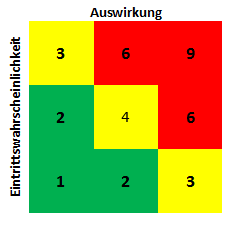
\includegraphics{Risikomatrix.png}
        \caption{Risikobewertung in einer 3x3 Matrix}
        \label{fig:riskmatrix}
    \end{figure}
    
    \clearpage
    \subsection{Massnahmenkatalog}
    Die Risiken mit einem Wert von 6 oder 9 werden als kritisch empfunden und erhalten eine Auflistung von Massnahmen gegen Auswirkung und Eintritt (Tabelle \ref{tab:arrangements}).
    \begin{table}[h]
        \centering
        \begin{tabular}{cp{7cm}p{7cm}}
            \textbf{RisikoNr} & \textbf{Massnahmen gegen Auswirkung} & \textbf{Massnahmen gegen Eintrittsw'keit}\\ \hline
            9 & \tabitem Alternative IDE für Debugging Zwecke & \tabitem Persönliche Präferenzen zurückstellen \\ \hline 
            13 & & \tabitem regelmässiges Reporting an die Stakeholder\\
            & &\tabitem gutes Requirementsengineering\\ \hline
            
        \end{tabular}
        \caption{Massnahmen gegen kritische Risiken}
        \label{tab:arrangements}
    \end{table}
    
    \clearpage
    %!TEX root = Projektdokumentation_ClockPendulumAnalyzer.tex
\section{Projektunterstützung}
Dieses Kapitel beschreibt die verwendeten Software zum Umsetzen der Arbeit.

\subsection{Tools für Entwicklung, Building und Deployment}
\begin{itemize}
    \item Für die Entwicklung der C++ Software wird das Entwicklerstudio CLion oder der klassische Texteditor VIM\footnote{programmierbarer Texteditor auf Linux} verwendet.
    \item Für die Entwicklung der C Software auf dem tiny K20 wird das Kinetis Design Studio (KDS) verwendet.
    \begin{itemize}
        \item Innerhalb von KDS wird der Processor Expert benutzt um Low-Level Ansteuerung für Register, Counter und Weiteres zu entwickeln.
    \end{itemize}
    \item Für die Entwicklung der Weboberfläche wird der klassische Texteditor VIM sowie Webstorm verwendet.
    \item Zum ''Builden'' der Software wird CMake Version 2.6 verwendet.
    \item Für das Deployment wird kein eigenes Tool verwendet. Die Software wird entweder direkt auf dem Target gebaut oder über die Entwicklungsumgebung auf das Target gespielt.
    \item Das Projektmanagement wird, ganz im Sinne einer agilen Planung, über die Onlineplattform ''Taigo.io'' abgehandelt.
\end{itemize}

    \clearpage
    %!TEX root = PMP_ClockPendelumAnalyzer.tex
\section{Test}
		\subsection{Testumgebung}
			\textit{in welcher Umgebung wurden die Tests gemacht}
		\subsection{Testfälle}
			\textit{Was wird durch das Testen abgedeckt}
			\subsubsection{Unit Tests}
			\subsubsection{Blackbox Tests}
	

\clearpage
\thispagestyle{empty}
	\section*{Anhang}
    %!TEX root = PMP_ClockPendulumAnalyzer.tex
\subsection*{Sprint 1}
Die Planung und der Abschluss von Sprint 1 ist in diesem Kapitel aufgeführt.
\subsubsection*{Planung}
Die Planung der Sprints wurde mit dem Programm Taiga.io durchgeführt. Unten ist ein Screenshot zu Beginn von Sprint 1.
    \begin{figure}[H]
        \centering
        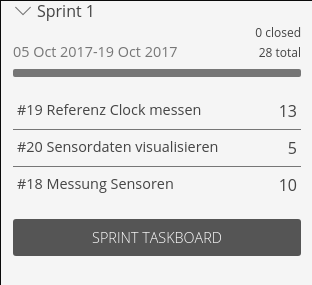
\includegraphics[width=.5\textwidth]{sprint1_plan.png}
        \caption{Sprintplanung für Sprint 1}
    \end{figure}
\subsubsection*{Abschlussprotokoll}
\end{document}
